\documentclass[10pt, landscape, a4paper]{article}
\usepackage{geometry}[landscape]
\usepackage{multicol}
\usepackage{graphicx}
\usepackage{amsmath} 
\usepackage{amssymb}
\usepackage{blindtext} % this can be removed later on

\usepackage[dvipsnames]{xcolor}
\usepackage{mathptmx}
\usepackage[compact]{titlesec}
\usepackage{paralist}

\usepackage{tabularx}
\usepackage{ctable}

% Set page margins
\geometry{top=0.2cm, left=0.2cm, right=0.2cm, bottom=0.2cm}

% Set indentation
\setlength{\parindent}{0pt}
\setlength{\parskip}{0.1cm}

% Set path for assets
\graphicspath{{assets/}}

\setlength{\columnsep}{5pt}
\raggedcolumns

% _____ CUSTOM COMMANDS __________________________________________
\newcommand{\E}[0]{\mathbb{E}}
\newcommand{\N}[0]{\mathbb{N}}
\newcommand{\R}[0]{\mathbb{R}}

\newcommand{\sgn}[0]{\text{sgn}}

\newcommand{\argmin}[1]{\underset{#1}{\text{argmin}}}
\newcommand{\argmax}[1]{\underset{#1}{\text{argmax}}}

\titlespacing{\section}{0pt}{0.5ex}{0ex}
\titlespacing{\subsection}{0pt}{0.5ex}{0ex}
%\linespread{0.9}

\newcommand*{\myfont}{\fontfamily{phv}\selectfont}

\newcommand{\greenbf}[1]{\textcolor{definitionColor}{\textbf{#1}}}
\newcommand{\bluebf}[1]{\textcolor{darkblue}{\textbf{#1}}}
\newcommand{\graytext}[1]{\textcolor{gray}{\footnotesize #1}}


% Define custom colors
\definecolor{darkblue}{RGB}{0, 0, 139}  % Adjust RGB values as needed
\definecolor{darkgreen}{RGB}{0, 100, 0}  % Adjust RGB values as needed
\definecolor{definitionColor}{rgb}{0,0.5,0}


\titleformat*{\section}{\fontsize{11}{11}\selectfont\myfont\bfseries\color{darkblue}}
\titleformat*{\subsection}{\fontsize{10}{10}\selectfont\myfont\bfseries\color{darkgreen}}
\begin{document}
\begin{multicols*}{4}

%\setlength{\abovedisplayskip}{0pt}
%\setlength{\belowdisplayskip}{0pt}
%\setlength{\abovedisplayshortskip}{0pt}
%\setlength{\belowdisplayshortskip}{0pt}

% _____ CONTENT __________________________________________________

% main heading
%\begin{center}
%	\Large{\te xtbf{Introduction to ML}} \\
%    \small{by dcamenisch}
%\end{center}



\section{The Digital Image}
\greenbf{Problems:} Transmission interference, compression artifacts, spilling, scratches, sensor noise, bad contrast and resolution, motion blur \\
\greenbf{Pixel:} Discrete samples of an continuous image function.\\
\greenbf{Rolling Shutter} effect produced by sequential readout of pixels while a digital camera is moving. Result is pixels read at different times are sequentially misaligned, causing image-level distortions dependent on camera (or object) movement.
\subsection*{Charge Coupled Device \graytext{(CCD)}}
Has an array of photosites \graytext{(a bucket of electrical charge)} that charge proportional to the incident light intensity during exposure. ADC happens line by line. \\
\greenbf{Bloooming:} oversaturation of finite capacity photosites causes the vertical channels to "flood" \graytext{(bright vertical line)}\\
\greenbf{Bleeding/Smearing:} While shifting down, the pixels above get some photons on bright spot with electronic shutters.\\
\greenbf{Dark Current:} CCDs produce thermally generated charge they give non-zero output even in darkness \graytext{(fluctuates randomly)} due to spontaneous generation of electrons due to heat $\rightarrow$ cooling.\\ can be avoided by cooling, worse with age.
\subsection*{CMOS:}
Same sensor elements as CCD, but each sensor has its own amplifier $\rightarrow$ faster readout, less power consumption, cheaper, more noise.\\ more noise, lower sensitivity\\
\greenbf{vs CCD} cheaper, lower power, less sensitive, per pixel amplification random pixel access, no blooming, on chip integration
\subsection*{Sampling methods}
Cartesian \graytext{(grid)}, hexagonal, non-uniform\\
\greenbf{Quantization:} Real valued function will get digital values \graytext{(integers)}. A lossy process \graytext{(original cannot be reconstructed)}. Simple version: equally spaced $2^b = \#bits$ levels\\
\greenbf{Linear Interpolation}: \\
$p(t) = p_0 + (t - t_0)\frac{p_1 - p_0}{t_1 - t_0} \text{ with } t \in [t_0, t_1]$ \\

\greenbf{Bilinear Interpolation:}     \\
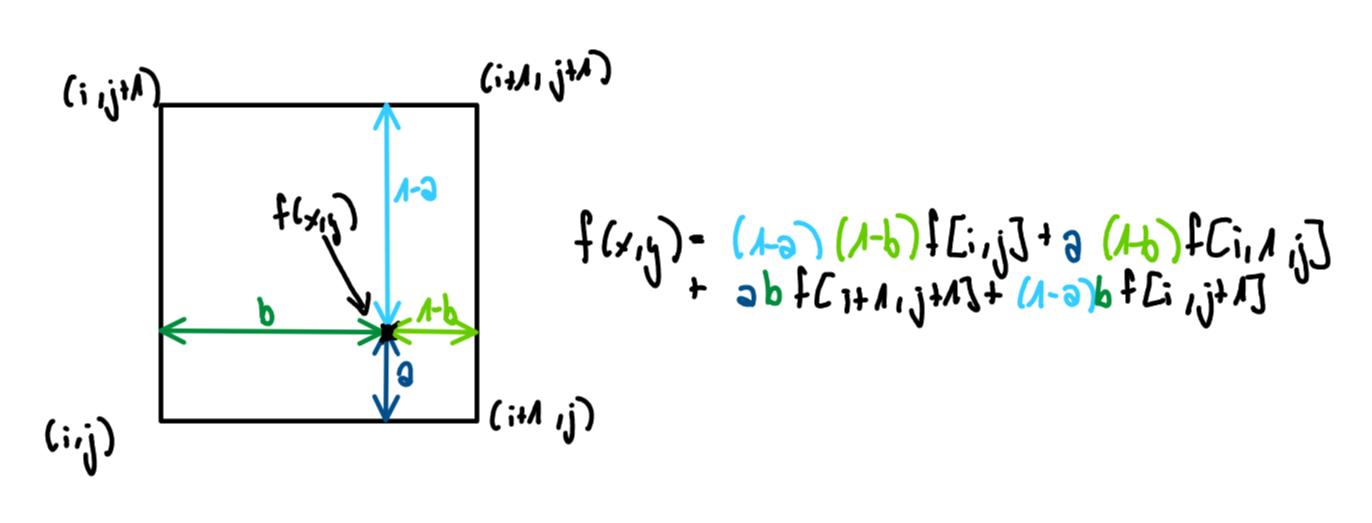
\includegraphics[width=\columnwidth]{jo/linear-interpolation.png} \\ 
\greenbf{Resolution:} Image resolution \graytext{(cropping)}, geometric resolution \graytext{(\#pixels per area)}, radiometric resolution \graytext{(\#bits per pixel, color)}\\
\greenbf{Image noise:} commonly modeled by additive Gaussian noise: $I(x, y) = f(x, y) + c$, poisson noise \graytext{(shot noise for low light, depends on signal \& aperture time)}, multiplicative noise: $I = f + f \cdot c$, quantization errors, salt-and-pepper noise. SNR or peak SNR is used as an index of image quality $c \sim N(0, \sigma^2)$, $p(c) = \frac{1}{\sigma \sqrt{2\pi}} \cdot \exp\left(-\frac{(c - \mu)^2}{2\sigma^2}\right)$, SNR: $S = \frac{F}{\sigma}$ where $F = \frac{1}{XY}\sum_{x = 1}^X \sum_{y = 1}^{Y} f(x, y)$.
\subsection*{Color cameras}
\greenbf{Prism} need 3 sensors and good alignment\\
\greenbf{Filter mosaic} coat $\square$ directly on sensor \\
\greenbf{Wheel} multiple filters in front of same sensor\\
\greenbf{New CMOS sensor} layers that absorb color at different depths $\rightarrow$ better quality
\section*{Image Segmentation}
\subsection*{Complete segmentation}
Finite set of non-overlapping regions that cover the whole image $I = \bigcup_{i = 1}^{n} R_i$ and $R_i \cap R_j = \emptyset$ $\forall i, j, i \neq j$\\
\greenbf{Thresholding:} simple segmentation by comparing greylevel with a threshold to decide if in or out.\\
\greenbf{Chromakeying:} when planning to segment, use special backgroundcolor. (Problems variations due to lighting, noise, ... mixed pixels (hard $\alpha$-mask does not work)) $I_\alpha = |I - g| > T$
\subsection*{Receiver Operating Characteristic (ROC) analysis:}
ROC curve characterizes performance of binary classifier Classification errors: False negative (FN), false positives (FP)\\
ROC curve plots TP fraction $\frac{TP}{TP + FN}$ vs FP fraction $\frac{FP}{FP + TN}$\\
\greenbf{Operating points:} choose point with gradient
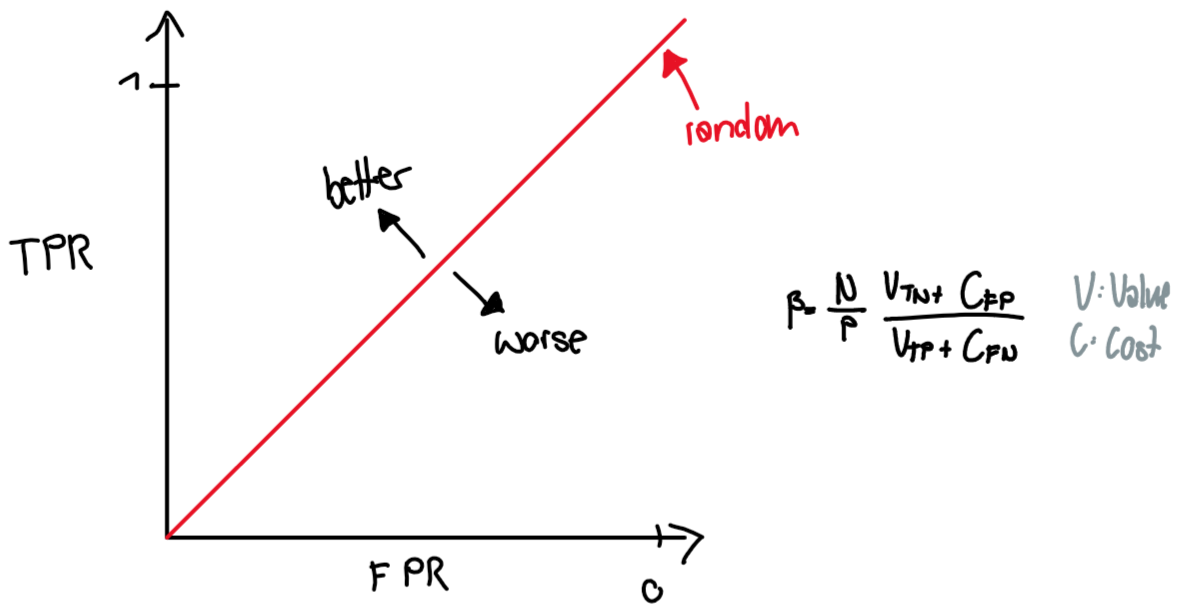
\includegraphics[width=0.4\columnwidth]{jo/roc.png} 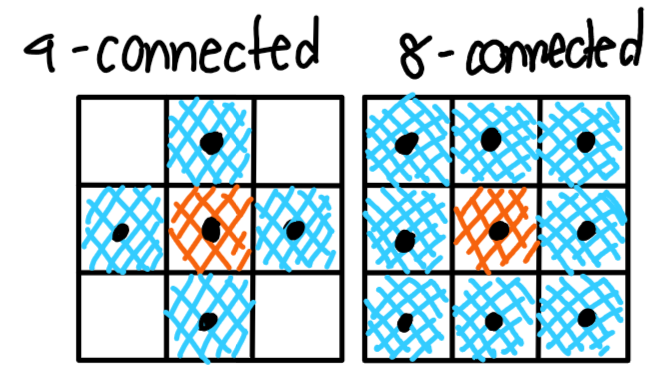
\includegraphics[width=0.4\columnwidth]{jo/connection.png}
\subsection*{Pixel connectivity}
\graytext{also regions if $x$-connected}\\
\greenbf{Connected component raster scanning:} scanning row by row, if foreground \& label if connected to other label, else give new label. (second pass to find equivalent labels)\\
\greenbf{Improve:} when region found, follow border, then carry on (contour-based method)
\subsection*{Region growing}
Start with seed point or region, add neighboring pixels that satisfy a criteria defining a region until we include no more pixels.\\
\greenbf{Seed region:} by hand or automatically by conservative Thresholding\\
\greenbf{Inclusion criteria:} greylevel thresholding, greylevel distribution model (include if ($I(x, y) - \mu^{2})^{2} < (n \sigma)^{2}$ and update $\mu$ and $\sigma$ after each iteration) color or texture information\\
\greenbf{Snakes:} active contour, a polygon and each point moves away from seed while criteria is met (can have smoothness constraint) Iteratively minimize enery function $E = E_{tension} + E_{stiffness} + E_{image}$
\subsection*{background subtraction}
simple: $I_\alpha = |I - I_{bg}| < T$ better: $I_\alpha = \sqrt{(I - I_{bg})^T \Sigma^{-1} (I - I_{bg})}$ where $\Sigma$ is the background pixel appearance covariance matrix, computed seperately for each pixel.
\subsection*{Morphological operators}
Logical transformations based on comparison of neighboring pixels\\
\greenbf{erode} delete FG pixels with 8-connected BG pixels\\
\greenbf{dilate} every BG pixels with 8-connected FG pixel make a FG pixel\\
\greenbf{Uses:} smooth regions, remove noise and artifacts.
\section{Image Filtering}
\greenbf{Local Filter:} A filter is local if it modifies pixels based on neighborhood.\\
Modify the pixels of an image based on some function of the local neighborhood of the pixels- If sum greater 1 get brighter, if smaller darker.\\
\greenbf{shift invariant:} Doing the same thing, applying the same function over all pixels (in the formula below if $K$ does not depend on $x, y$)\\
\greenbf{Linear Filtering}\\
$L$ is linear operation if $L[\alpha I_1 + \beta I_2] = \alpha [I_1] + \beta L[I_2]$\\
\greenbf{Linear:} linear combination of neighbors can be written as: \\
$\sum_{\begin{subarray}{c}
    (i, j) \in \underbrace{\mathbb{N}(x, y)}_{\text{neighborhood}}
\end{subarray}}
K(x, y, i, j) \underbrace{I}_{\text{Input}} (x + i, y + j)$

\greenbf{Filter at edges:} clip filter (black), wrap around, copy edge, reflect across edge, vary filter near edge
\subsection*{Correlation}
$I'(x, y) = \sum_{(i, j) \in \N(x, y)} K(i, j) I (x + i, y + j)$ \\
$I' = K \circ I \quad$ e.g. template matching: search for best match by minimizing mean squared error or maximizing area correlation. (remove mean (from filter, from image) to avoid bias)
\subsection*{Convolution}
$I' = K * I, I'(x, y) = \sum_{(i, j) \in \N(i, j)} K(i, j) I (x - i, y - j)$ if $K(i, j) = K (-i, -j) \implies \\
correlation = convolution \quad\\
convoution = correlation + \text{ filter rotated 180°}$\\
\greenbf{Continuous:} $(f * g)(t) \\
= \int_{-\infty}^{\infty} f(\tilde{t}) g(t - \tilde{t}) d\tilde{t}\\
= \int_{-\infty}^{\infty} f(t - \tilde{t}) g(\tilde{t}) dt$
\subsection*{Kernels}
\greenbf{separable:} if a kernel can be written as a product of two simpler filters $\rightarrow$ computationally faster (filter $P \times Q$, image $N \times M: (P + Q) * NM$ instead of $PQNM$)\\
Separable filters can be written as \( K(m,n) = f(m)g(n) \).
For a rectangular neighborhood with size \((2M+1) \times (2N+1), I'(m, n) = \fcolorbox{green}{white}{f * (\fcolorbox{red}{white}{g * I(N(m, n))})}\)\\
$
\fcolorbox{red}{white}{I''(m,n)} = \sum_{j=-N}^{N} g(j) I(m, n - j)
$
\\
$\fcolorbox{green}{white}{I'(m, n)} = \sum_{j=-N}^{N} f(i) I''(m - i, n)$\\
\greenbf{Box filter:} all same values normalized to sum = 1\\
\greenbf{Gaussian Kernel:} $K(x, y) = \frac{1}{2\pi \sigma^{2}} e^{-\frac{x^{2} + y^{2}}{2\sigma^{2}}}$ is separable, e.q. $\sigma = 1$\\
Gaussian Smoothing Kernel Top-5
\begin{compactitem}
\item Rotationally symmetric
\item has single lobe \graytext{Neighbor's influence decreases monotonically}
\item Still one lobe in frequency domain ,\graytext{No corruption from high frequencies}
\item Simple relationship to $\sigma$
\item Easy to implement efficiently
\end{compactitem}
\greenbf{High Pass Filter:}
high pass filter detects edges 
High Pass Filter Laplacian Operator \\
$
\begin{bmatrix}
   % \begin{smallmatrix}
        -1 & -1 & -1 \\
        -1 & 8 & -1 \\
        -1 & -1 & -1 \\
    %\end{smallmatrix}
\end{bmatrix} 
$$
\begin{bmatrix}
    %\begin{smallmatrix}
        0 & 1 & 0 \\
        1 & -4 & 1 \\
        0 & 1 & 0 \\
    %\end{smallmatrix}
\end{bmatrix} 
$
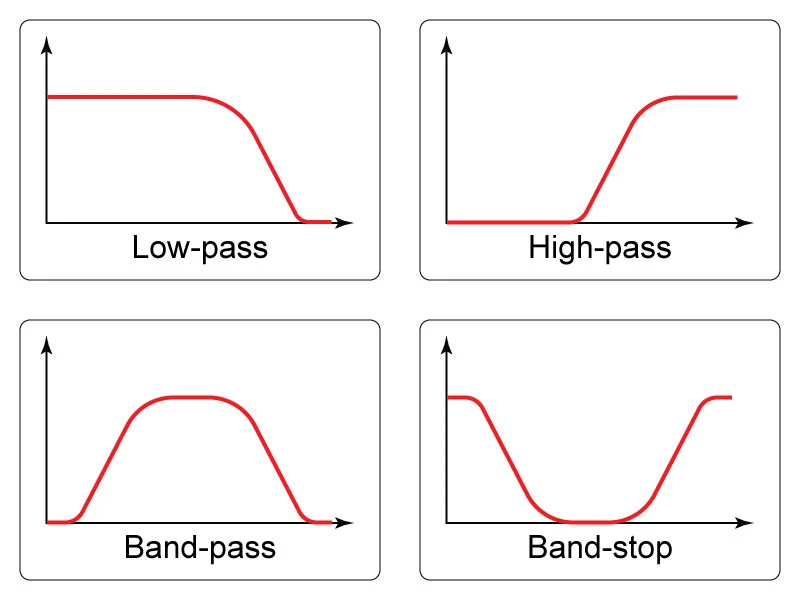
\includegraphics[width = 0.3 \columnwidth]{assets/jo/Types_of_Filters.png}

\greenbf{Low Pass Filter:}
blurs (detects "smooth" regions) Gaussian Filter is a low pass filter, proof: Convolution theorem: Fourier transform H of h is equal to $F \cdot G$
If $g$ is Gaussian, its Fourier Transform $G$ is also Gaussian.
Pointwise multiplication of $F$ with $G$ will keep the low frequencies of F unchanged, while the high frequencies will be multiplied by a low number, and therefore, they will be removed.  \\
\greenbf{Conversion:} Subtracting one from central element of low-pass filter gives a high-pass filter with inverted sign, because.\\
$(f - \delta) * a = f * a - \delta * a = f * a - a = - (a - (f * a))$ Normalize the low-pass kernel and then subtract one from central element. Normalize low-pass filter, then subtract the kernel from central element matrix. To get the high pass filter, you do not need to normalize.\\
\greenbf{Band pass filter:} 
\includegraphics*[width = 0.4cm]{jo/band-pass-filter.png}
do LPF and HPF with cutoffs $f_{LP} < f_{HP} \quad f = \text{ cut of frequencies, cannot coincide}$\\
Filter image with high-pass and low-pass filter to get band pass filter. \graytext{Only works when you have an overlap in frequencies. If no overlap: $I *_{convolution} (\delta - f_{LP - f_{HP}}) \rightarrow $ gap between is band filter.}\\
\greenbf{Band reject filter:} \includegraphics*[width = 0.4cm]{jo/band-reject-filter.png}
do LPF and HPF with cutoffs $f_{LP} > f_{HP}$\\
\greenbf{Image sharpening:} increases high frequency components to enhance edges: $I' = I + \alpha |K * I|$ $K:$ high-pass filter, $\alpha$: scalar $\in [0, 1]$
\section{Features}
\greenbf{Desirable properties:} shift, rotation, scale, brightness invariant
\subsection*{Edge Detection}
How to tell if there is an edge? Local maxima of the first derivative and the zero crossing of the second derivative.\\
\greenbf{Edge detection filters:}

\greenbf{Sobel:}\\
$K_x = \begin{bmatrix}
    \begin{smallmatrix}
        -1 & 0 & 1\\
        -2 & 0 & 2\\
        -1 & 0 & 1
    \end{smallmatrix}
\end{bmatrix}$,
$K_y = \begin{bmatrix}
    \begin{smallmatrix}
        -1 & -2 & -1\\
        0 & 0 & 0\\
        1 & 2 & 1
    \end{smallmatrix}
\end{bmatrix}$

\greenbf{Prewitt:}\\
$K_x = \begin{bmatrix}
    \begin{smallmatrix}
        -1 & 0 & 1\\
        -1 & 0 & 1\\
        -1 & 0 & 1
    \end{smallmatrix}
\end{bmatrix}$,
$K_y = \begin{bmatrix}
    \begin{smallmatrix}
        -1 & -1 & -1\\
        0 & 0 & 0\\
        1 & 1 & 1
    \end{smallmatrix}
\end{bmatrix}$

\greenbf{Roberts:}\\
$K_x = \begin{bmatrix}
    \begin{smallmatrix}
        1 & 0\\
        0 & -1
    \end{smallmatrix}
\end{bmatrix}$,
$K_y = \begin{bmatrix}
    \begin{smallmatrix}
        0 & 1\\
        -1 & 0
    \end{smallmatrix}
\end{bmatrix}$

\greenbf{Gradient Magnitude:}\\
$M(x, y) = \sqrt{(\frac{\partial f}{\partial x})^{2} + (\frac{\partial f}{\partial y})^{2}}$\\
\greenbf{Gradient Angle:} \\
$\alpha(x, y) = \tan^{-1}(\frac{\partial f}{\partial y} / \frac{\partial f}{\partial x})$
\subsection*{Laplacian operator}
detect discontinuities by considering second derivative
$\begin{bmatrix}
    \begin{smallmatrix}
        0 & 1 & 0\\
        1 & -4 & 1\\
        0 & 1 & 0
    \end{smallmatrix}
\end{bmatrix}
\quad \text{or} \quad
\begin{bmatrix}
    \begin{smallmatrix}
        1 & 1 & 1\\
        1 & -8 & 1\\
        1 & 1 & 1
    \end{smallmatrix}
\end{bmatrix}$
are discrete space approximations. Is isotropic\graytext{(rotationally invariant)}, zero crossings make edge locations. Sensitive to fine details and noise \graytext{($\rightarrow$ smoothing before applying)}.\\ blur image first \graytext{(LoG)}\\
\greenbf{Laplacian of Gaussian \graytext{(LoG)}:} convolve gaussian blurring and laplacian operator in LoG operator \graytext{(cheaper)} $LoG(x, y) = -\frac{1}{\pi \sigma^{4}} (1 - \frac{x^{2} + y^{2}}{2\sigma^{2}}) e^{-\frac{x^{2} + y^{2}}{2\sigma^{2}}}$
\subsection*{Canny Edge Detector: 5 Steps}
\begin{compactenum}
    \item smooth image with a Gaussian filter
    \item compute gradient magnitude and angle using Sobel/Prewitt/...
    \item apply non-maximum suppression to gradient magnitude image \graytext{(Quantize edge normal to one of four directions: horizontal, +45°, vertical, -45°. If $M(x, y))$ smaller than either of its neighbors in edge normal direction suppress, else keep}
    \item Double thresholding for intensity to detect strong and weak edge pixels
    \item Reject weak edge pixels not connected to strong edge pixels
\end{compactenum}
\subsection*{Hough Transform}
Fitting a straight line to a set of edge pixels\\
\includegraphics*[width = \columnwidth]{jo/slope.png}\\
\greenbf{Alternative parameterization:}\\
$x \cos(\theta) + y \sin(\theta) = \rho$ \\
$(x - a)^{2} + (y - a)^{2} = r^{2}$
\greenbf{For circles:} if r known: calculate circles with radius r around edge pixels $\rightarrow$ intersection (local maxima) of circles gives center.\\ Where lots of them meet is the center of a circle. else: use 3D hough transform with parameters $(x_0, y_0, r)$
Each point $(x_i, y_i)$ in the $xy$-plane gives a sinusoid in the $\theta \rho$ plane. Colinear points lying on the line give curves intersecting at the same point in the polar parameter plane. Local maxima give significant lines.
\subsection*{Corner Detection}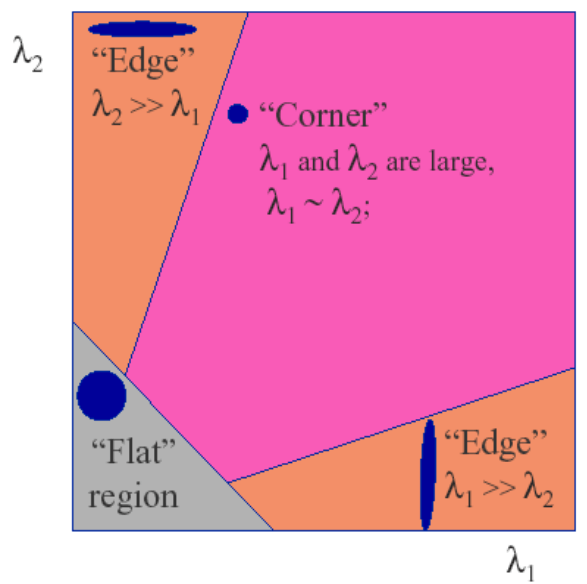
\includegraphics[width = 2cm]{jo/corner.png}\\
Edges are only well localized in one direction $\rightarrow$ detect corners.\\
Desirable properties: Acute localization, invariance against shift, rotation, scale, brightness change, robust against noise, high repeatability\\
\greenbf{Linear approximation for small $\Delta x \Delta y$:} (Taylor) $f(x + \Delta x, y + \Delta y) \approx f(x, y) + f_x(x, y) \Delta x + f_y(x, y)\Delta y$
\subsection*{Local displacement sensitivity \graytext{(Harris corners)}}
$S (\Delta x, \Delta y) = (\Delta x \Delta y) \left( \sum_{x, y \in \text{window}}
\begin{bmatrix}
    \begin{smallmatrix} 
        f_x^{2} & f_x f_y \\ 
        f_x f_y & f_y^{2} 
    \end{smallmatrix} 
\end{bmatrix}
\right)
\begin{bmatrix}
    \begin{smallmatrix} 
        \Delta x \\ 
        \Delta y
    \end{smallmatrix} 
\end{bmatrix}  \\
\approx \text{SSD}$.
Find points where $\min \Delta^T M \Delta$ is large for $||\Delta || = 1$ i. e. maximize the eigenvalues of $M$\\
\greenbf{Harris cornerness:} Measure of cornerness\\
$C(c, y) = \det(M) - k * trace(M)^{2} = \lambda_1\lambda_2 + k(\lambda_1 + \lambda_2)$ \\
\greenbf{Robustness of Harris corner detector:} Invariant to brightness offset, invariant to shift and rotation but not to scaling!
$\lambda_1 >> \lambda_2 \rightarrow$ edge, $\lambda_1$ and $ \lambda_2$ large $\rightarrow$ corner, else $\rightarrow$ flat region.\\
not scale invariant: \includegraphics*[width = 4cm]{jo/corner-edge.png}\\
\greenbf{Overcome issues:} look for strong DoG response or consider local maxima in position and scale space, Gaussian weighing.
\subsection*{Lowe's SIFT features}
Look for strong responses of difference of Gaussians \graytext{(DoG)} filter, only look at local maxima in both position and scale.\\
\greenbf{DoG:} $DoG(x, y) = \frac{1}{k}* e^{-\frac{x^{2} + y^{2}}{(k\sigma)^{2}}} - e^{-\frac{x^{2} + y^{2}}{\sigma^{2}}}$ e.g. $k = \sqrt{2}$\\
Orientation: create histogram of local gradient directions computed at selected scale, assign canonical orientation at peak of smoothed histogram. Get a SIFT descriptor \graytext{(threshold image gradients are sampled over $16\times 16$ array of locations in scale space)} and do matching with these. Invariant to scale, rotation, illumination and viewpoint.



\section{Fourier Transformation}
\greenbf{Aliasing:} Happens when undersampling e.g. taking every second pixel, else characteristic errors appear: typically small phenomena look bigger, fast phenomena look slower. (e.g. wagon wheels backwards in movies, checkerboards misrepresented)
\subsection*{Fourier Transform}
\greenbf{Convolution, Filtering:} The Fourier transform of the convolution of two functions is the product of their Fourier transform:\\
$F \cdot G = U(f ** g)$\\
\greenbf{Convolution, Sampling:} The Fourier transform of the product of two functions is the convolution of the Fourier transform.\\
$F ** G = U(f \cdot g)$\\
%$\sin(x) = \frac{e^{ix} - e^{-ix}}{2i}$\\
%$\cos(x) = \frac{e^{ix} + e^{-ix}}{2}$\\
Represent function on a new basis with basis elements $e^{i 2 \pi (ux + vy)} = \cos(2 \pi (ux + vy)) + i \sin(2 \pi (ux + vy))$\\
$F(f(x))(u) = \int_{-\infty}^{\infty} f(x) e^{-i 2 \pi ux} dx$, \\
\greenbf{Inverse Fourier:} $f(x) = \int_{\infty}^{\infty} F(u)e^{i2\pi ux} du$ Similar for 2D \\
\greenbf{2D:} $F(f(x,y))(u, v) = \int_{-\infty}^{\infty} \int_{-\infty}^{\infty} f(x, y) e^{-2\pi i (ux + vy)}dx dy$\\
\greenbf{For images:} transformed image $\rightarrow$ $F = U * f$ $\leftarrow$ vectorized image, U: Fourier matrix\\
\greenbf{For discrete:} \\$F(u, v) = \frac{1}{NM}\sum_{x=0}^{N-1} \sum_{y=0}^{M-1} f(x, y) e^{-2\pi i (\frac{ux}{N}, \frac{vy}{M})}$\\ % source: Processing Signals Slide 15
\greenbf{1D-periodic function:} $f(t) = \sum_{n = -\infty}^{\infty} c_n e^{\frac{i 2 \pi n t}{T}}$, $c_n = \frac{1}{T} \int_{-\frac{T}{2}}^{\frac{T}{2}} f(t) e^{\frac{-i 2 \pi n t}{T}} dt$
\subsection*{Properties of Fourier transform}
\greenbf{Linearity:} $F(ax(t) + by(t)) = aX(t) + bY(t)$\\
\greenbf{Time Shift:} $F(x(t \pm t_0)) = X(t) e^{\pm i 2 \pi f t_0}$\\
\greenbf{Frequency Shift:} $F(e^{i 2 \pi f_0 t} x(t)) = X(f - f_0)$\\
\greenbf{Scaling:} $F(x(at)) = \frac{1}{|a|}X\left(\frac{f}{a}\right)$\\
\greenbf{Convolution:} $F(x(t) * y(t)) = X(f) \cdot Y(f)$\\
\greenbf{Duality:} $F(X(t)) \longleftrightarrow x(-f)$

\color{definitionColor}
\greenbf{Sampling:} \color{black}

A sampling function $s(t)$ which is an impulse train with period $T$ and its Fourier transform $S(f)$:\\
\color{gray}
$s(t) = \sum_{n = -\infty}^\infty \delta\left(t - nT\right)$\\
$ S(f) = \frac{1}{T} \sum_{n = -\infty}^\infty X(f - \frac{n}{T}) \text{ where } \delta(*) \text{  Dir.-delt. f.}$\\
\color{black}
A continuous signal can be sampled by multiplying with $s(t):$ \graytext{$x_s(t) = x(t)s(t)$}To compute the Fourier Transform of $x_s(t)$, we can use the convolution theorem:

\graytext{
$F(x_s(t)) = X(t) * S(t) = \frac{1}{T}\sum_{n = -\infty}^\infty \delta\left(f - \frac{n}{T}\right) * X(t) = \frac{1}{T}\sum_{n = -\infty}^\infty X(f - \frac{n}{T})$
}

\greenbf{Sampling in 2D:} $sample_{2D} (f(x, y)) = \sum_{i = \infty}^{\infty} \sum_{j = \infty}^{\infty} f(x, y) * \delta(x - i, x - j) = f(x, y) \sum_{i = \infty}^{\infty}\sum_{j = \infty}^{\infty}\delta(x - i, x - j)$

\greenbf{DFT:} 
The 2D DFT of an image \( I(x, y) \) is given by:
$F(u, v) = \sum_{x=0}^{N-1} \sum_{y=0}^{N-1} I(x, y) \cdot e^{-j2\pi\left(\frac{ux}{N} + \frac{vy}{N}\right)} $
$ F(f(x, y))  (\sum_{i = \infty}^{\infty}\sum_{j = \infty}^{\infty}\delta(x - i, x - j)) F(f(x, y)) * F( \sum_{i = \infty}^{\infty}\sum_{j = \infty}^{\infty}\delta(x - i, x - j)) =  \sum_{i = \infty}^{\infty}\sum_{j = \infty}^{\infty} F(u - i, v - j)$

\greenbf{Dirac Delta Function:} \\
$\delta (K - k) =  \int_{-\infty}^{\infty}e^{2 \pi i(K - k)x} dx$

$\int_{-\infty}^{\infty} \delta(t) \, dt = 1 \quad \text{and} \quad \delta(t) =  \begin{cases} 0 & \text{ for } x \neq 0 \\ und. & \text{ for } x = 0 \end{cases}$

\greenbf{Sifting Property:}

\color{black} 
$\int_{-\infty}^{\infty} f(t) \cdot \delta(x - a) \, dx = f(a)$

\greenbf{Dirac Comb:} 

$\text{III}_T(x) = \sum_{n=-\infty}^{\infty} \delta(t - nT)$\graytext{sampling = product with this}

\greenbf{Box Filter:}
$h(x) = \begin{cases} 
\frac{1}{T}, & \text{if } |x| \leq \frac{T}{2} \\ 0, & \text{otherwise.} \end{cases}$

$f_{recon} = (h*g)(x) =\\
T \int_{-\infty}^{\infty} h(y) \sum_{i = -\infty}^{\infty} f(iT) \delta(x-y-iT)dy$\\
\greenbf{Triangle Filter:}
$\text{tri}(t) = \begin{cases} 1 - |t|, & \text{if } |t| \leq 1 \\ 0, & \text{otherwise.} \end{cases}$

\subsection*{Fourier transform of important functions}
\includegraphics*[width = \columnwidth]{jo/fourier-transform-important-functions.png}
\subsection*{Nyquist Sampling theorem}
The sampling frequency must be at least twice the highest frequency $w_s \geq 2 w$ \graytext{If not the case: band limit before with low-pass filter. Perfect reconstruction: $sinc(x) = \frac{sin(\pi x)}{\pi x}$}

\greenbf{Why should this hold?} \graytext{Function $f(t)$, sampling function $S_{\Delta t}(t)$ with sampling frequency $w_s$}. Fourier transform of the sampled function can be derived as
$
\tilde{F}(u) = F(f(t) \cdot S_{\Delta t}(t)) \\
            = F(u) * S_{\Delta t}(w) \\
            = \int_{-\infty}^{\infty} F(\tilde{t}) S_{\Delta t}(w - \tilde{t}) \, d\tilde{t} \\
            = \int_{-\infty}^{\infty} F(\tilde{t}) \frac{1}{\Delta T} \sum_{n = -\infty}^{\infty} \delta (w - \tilde{t} - \frac{n}{\Delta T}) \, d\tilde{t} \\
            = \frac{1}{\Delta T} \sum_{n = -\infty}^{\infty} F(w - n w_s).
$\\
If we want to reconstruct the signal $f(t)$ from $F$ and $S_{\Delta t}$, $F(w)$ cannot overlap with its neighbors $F(w - w_s)$ and $F(w + w_s)$. Thus, $w_s$ should be larger than $w_n$. \graytext{Highest frequency of $f(t)$}.
\subsection*{Image restoration problem: $f(x) \rightarrow h(x) \rightarrow g(x) \rightarrow \tilde{h}(x) \rightarrow f(x)$}
The "inverse" kernel $\tilde{h}(x)$ should compensate $h(x)$. May be determined by: $F(\tilde{h})(u, v) \cdot F(h(u, v)) = 1$\\
\greenbf{Problems:} Convolution with kernel $k$ may cancel out some frequencies \& noise amplification. \\
\greenbf{Avoid:} Regularization: $F(\tilde{h})(u, v) = \frac{F(h)}{{|F(h)|}^{2} + \epsilon}$ \graytext{avoid singularities}

\section{Optical Flow}
Apparent motion of brightness patterns use extracted feature points and commpute their velocity vectors \graytext{projection of 3D velocity vectors on I}\\
\greenbf{Problem:} cannot distingish motion from changing lighting! also estimate observed projected motion field \graytext{normal flow} not always well defined \\
\greenbf{Key assumptions:} \\
Brightness constancy: \graytext{Proection of the same point looks the same in every frame.}\\
Small motion: \graytext{Points do not move far}\\
Spatial coherence: \graytext{Points move like their neighbors}\\
\greenbf{Brightness constancy constraint:} $I(x, y, t - 1) = I(x + u, y + v, t) I = Intensity$\\
Small motion $\rightarrow$ can linearize with Taylor expansion:\\
\graytext{$I(x, y, t - 1) \approx I(x, y, t - 1) + \frac{\partial I}{\partial x} u + \frac{\partial I}{\partial y} v + \frac{\partial I}{\partial t} \approx 0$} or shorthand \graytext{$I_x \cdot u + I_y \cdot v + I_t \approx 0$}\\
move $I-t$ on one side, vectorize unknowns. For LK, sum up over a window of pixes\\
\greenbf{Apature problem:} 1 equation, 2 unknowns cannot determine exact location, take normal flow. \includegraphics*[width =0.6 \columnwidth]{jo/feature.png}\\
Add additional smoothness constraint: \\
\graytext{$e_s = \int \int (u_x^2 + u_y^2 + v_x^2 + v_y^2) dxdy$ $close \approx parallel$}\\
Besides OF constraint: \\
\graytext{$e_c = \int \int (I_x u + I_y v + I_t)^2 dxdy$} Minimize $e_s + \lambda e_c$
\subsection*{Lukas-Kanade}
Assume same displacement for $N \times M$ window $\rightarrow$ linear least squares problem:
\graytext{$\begin{bmatrix}
    \begin{smallmatrix}
        I_x(x_1, y_1) & I_y(x_1, y_1)\\
        \vdots & \vdots\\
        I_x(x_{NM}, y_{NM}) & I_y(x_{NM}, y_{NM})
    \end{smallmatrix}
\end{bmatrix}
\begin{bmatrix}
    \begin{smallmatrix}
        u\\
        v
    \end{smallmatrix}
\end{bmatrix}
= -\begin{bmatrix}
    \begin{smallmatrix}
        I_t(x_1, y_1)\\
        \vdots\\
        I_t(x_{NM}, y_{NM})
    \end{smallmatrix}
\end{bmatrix} \implies 
\begin{bmatrix}
    \begin{smallmatrix}
        \sum I_x I_x & \sum I_x I_y\\
        \sum I_y I_x & \sum I_y I_y
    \end{smallmatrix}
\end{bmatrix}
\begin{bmatrix}
    \begin{smallmatrix}
        u\\
        v
    \end{smallmatrix}
\end{bmatrix}
= -\begin{bmatrix}
    \begin{smallmatrix}
        \sum I_x I_t\\
        \sum I_y I_t
    \end{smallmatrix}
\end{bmatrix}$}\\
\greenbf{When solvable?} $A^TA$ invertible, eigenvalues $\lambda_1, \lambda_2$ large, $\frac{\lambda_1}{\lambda_2}$ small\\
\greenbf{Errors:} motion is large\graytext{(r than a pixel) \\
$\rightarrow$ iterative refinement and coarse-to-fine estimation.} \\
A point does not move like its neighbors \\
\graytext{$\rightarrow$ motion segmentation.}\\
Brightness constancy does not hold:\\
 \graytext{$\rightarrow$ exhaustive neighborhood search with normalized corrolation.}\\
\greenbf{KLT feature tracker:} to find patches where LSE well-behaved $\rightarrow$ LK-flow\\
\greenbf{Iterative refinement:} Estimate velocity, warp using estimate, refine,...\\
\greenbf{Coarse-toFine Estimation:} Image Pyramid. Start small, compute OF, rescale, take larger and initialize with last estimate\\
\greenbf{Applications:} Image stabilization \graytext{(get flow between two frames and warp image using same OF for all pixels s.st. OF close to 0)} frame interpolation, video compression, object tracking, motion segmentation\\
\greenbf{Affine motion:} $I_x(a_1 + a_2x + a_3y) + I_y(a_4 + a_5x + a_6y) + I_t \approx 0$ \includegraphics*[width = 0.75 \columnwidth]{jo/planes.png}\\
\greenbf{SSD tracking:} For large displacements: match template against each pixel in small area around, match measure can be (normalized) correlation or SSD choose max. as match \graytext{(sub-pixel also possible)}\\
\greenbf{Bayesan Optical Flow:} Some low-level motion illusions can be explained by adding an underlying model to LK-tracking e.g. brightness constancy with noise.

\section{Video Compression}
\greenbf{Interlaced video format:} 2 temporally shifted half images \\
\graytext{$\rightarrow$ increase frequency, decrease spatial resolution} $\rightarrow$ not progressive\\
\greenbf{Lossy video compression:} take advantage of redundancy spatial correlation between pixels, temporal correlation between frames \\
\graytext{$\rightarrow$ basically drop perceptually unimportant details}\\
\greenbf{with optical flow:} Encode optical flow based on previous frame can cause blocking artifacts, does not work well for lots of movemen, fast movement and scene changes.\\
\graytext{If temporal redundancy fails $\rightarrow$ use motion-compensated prediction}\\
\greenbf{Types of coded frames:}\\
\bluebf{I-Frame:} Intra-coded frame, coded independently of all others\\
\bluebf{P-Frame:} Predictively coded frame, based on previously coded frame\\
\bluebf{B-Frame:} Bi-directionally coded frame, based on previous \& future
\subsection*{Block-Matching Motion Estimation:}
Is a type of temporal redundancy reduction\\
\greenbf{Motion Estimation Algorithm \graytext{ME}}
\begin{compactenum}
    \item Partition frame into blocks (e.g. $16 \times 16$ pixels)
    \item For each block, find the best matching block in reference frame
\end{compactenum}
Metrics for best match: \graytext{sum of differences or squared sum of diff.}\\
Candidate blocks: \graytext{All blocks in e.g. $32 \times 32$ pixel area}\\
Search strategies: \graytext{Full search, partial (fast) search}\\
\greenbf{Motion Compensation Algorithm \graytext{MC}}
Use the best matching of reference frame as prediction of blocks in current frame\\
\graytext{$\rightarrow$ gives motion vectors \& MC prediciotn error or residual (encode with conventionl image coder)}\\
\greenbf{Motion Vector:} relative horizontal \& vertical offsets of a given block from one frame to another\\
\graytext{Not limited to integer-pixel offsets, can use half-pixel ME to capture sub-pixel motion.}\\
\greenbf{Half-pixel ME (coarse-fine) algorithm:}
\begin{compactenum}
    \item Coarse step: find best integer move
    \item Fine step: refine by spatial interpolation and best-matching
\end{compactenum}
\greenbf{Advantages and disadvanages}\\
+ good, robust performance, one MV per block $\rightarrow$ useful for compression, simple periodic structure \graytext{(GoP)}\\
- assumes translational motion (fails for complex motion)\\
\graytext{$\rightarrow$ codes these frames/blocks without prediction} produces blocking artifacts\\
\greenbf{MPEG-GoP} IBBPBBPBBI dependencies between frames
\subsection*{Scalable Video Coding:}
Decompose video into multiple layers of prioritized importance: e.g. \\
temporal scalability: \graytext{Include B-frames or not}\\
spatial scalability: \graytext{Base resolution + upsampling difference}\\
SNR scalability: \graytext{Base with coarse quatizer + fine quantizer}\\
\greenbf{Benefits:} Adapting to different bandwidths, facilitates error resiliency by identifying more and less important bits.
\section{Unitary Transforms}
\greenbf{Vectorization:} interpret image as vector row-by-ow: \graytext{$I = \begin{bmatrix}
    \begin{smallmatrix}
        1 & 2 & 3\\
        4 & 5 & 6
    \end{smallmatrix}
\end{bmatrix} \rightarrow \begin{bmatrix}
    \begin{smallmatrix}
        1 & 2 & 3 & 4 & 5 & 6
    \end{smallmatrix}
\end{bmatrix}$}\\
\greenbf{linear image processing:} can be written as $\vec{g} = H\vec{f}$\\
\greenbf{Image collection (IC):} $F = [f_1, f_2... f_n]$\\
\greenbf{Autocorrelation matrix} $Rff = \frac{F \cdot F^H}{N}$ its Eigenvector with largest Eigenvalue is direction of largest variance among pictures.\\
\greenbf{Unitary transform:} for transform $A$ iff $A^H = A^{-1}$ \graytext{if real-valued $\rightarrow$ orthonormal}\graytext{every unitary transform is a rotation + sign flip, length conserved}\\
\greenbf{Energy conservation:} $||\vec{C}||^{2} = \vec{C}^{H}C = \vec{f}^{H}A^{H}Af = ||\vec{f}||^{2}$ \\
\subsection*{Karhunen-Loeve Transform \graytext{Same as PCA. Order by decreasing eigenvalues}}
\greenbf{Energy concentration property:} no other unitary transform packs as much energy in the first $J$ coefficients \graytext{(for arbitrary $J$)} and mean squared approximation error by choosing only first $J$ coefficients is minimized.\\
\greenbf{Optimal energy concentratioin of KLT} consider truncated coefficient vector $\vec{b} = I_J \vec{c}$ \graytext{($I_J$: identity matrix with first J columns)} Energy in first $J$ coefficients for an arbitrary transform $A : E = Tr(R_{bb}) = Tr(I_J R_{cc} I_{J}) = Tr(I_J A R_{ff} A^H I_J) = \sum_{k = 0}{J = 1} a_k^T R_{ff} a_k^*$ where $a_k^T$ is $k-th$ row of $A$. Lagrangian cost function to enforce unit-length basis vectors: 
$L = E + \sum_{k = 0}^{J - 1} \lambda_k (1 - a_k^T a_k^*) = \sum_{k = 0}^{J - 1} a_k^T R_{ff} a_k^* + \sum_{k = 0}^{J - 1} \lambda_k (1 - a_k^T a_k^*)$\\ 
Differentiating $L$ with respect to $a_j$: $R_{ff} a_j^* = \lambda_i a_j^* \quad \forall_j < J$ \graytext{necessary condition}
\subsection*{Simple recognition}
SSD between images, best match wins \graytext{very expensive, since need to correlate with every image}
\subsection*{Principle Component analysis \graytext{PCA}}
\greenbf{Steps:} standardize data, get Eigenvectors and values from covariance matrix or do SVD, sort Eigenvalues and vectors in descending order get $j$ largest components, construct projection matrix from selected $j$ Eigenvectors transform dataset by multiplying with projection matrix.\\
\includegraphics*[width = 0.4\columnwidth]{jo/pca.png}\\
\greenbf{Uses of PCA:} lossy compression by keeping only the most important $k$ components. Face recognition \graytext{eigenfaces} and face detection.
\subsection*{Eigenspace matching}
Do PCA \graytext{with mean subtraction} and get closest rank-$k$ approximation of database images \graytext{(eignfaces)} \\
For a new query: normalize, subtract mean \graytext{(of database)} project to subspace then do similarity matching with eigenfaces.
\subsection{Fischerfaces:} 
Find directions where ratio between / within individual variance is maximized. Linearly project to basis where dimension with good signal: noise ratio is maximized. \\
$W_{\text{opt}} = \argmax{W} \frac{\det(W R_B W^H)}{\det(W R_W W^H)}, R_b = \sum R_B \sum_{i = 1}{c} N_i (\vec{\mu_i} - \vec{\mu})(\vec{\mu_i} - \vec{\mu})^H, R_W = \sum_{i = 1}^{c} \sum_{\Gamma_l \in Class} (\Gamma_l - \mu_i)(\Gamma_l - \mu_i)^H$\\
\greenbf{Fischer linear discriminant analysis \graytext{(LDA)}:} maximize between class scatter, while minimizing within less scatter
\subsection*{JPEG Compression}
Divide image into $8 \times 8$ block:\\
\includegraphics*[width = \columnwidth]{jo/jpg.png}\\
\greenbf{DC:} First coefficient (general intensity)\\
\greenbf{ZigZag:} \includegraphics*[width = 1.5cm]{jo/zig-zag.png}\\
\greenbf{Quantization Table:} Divide by this value, round to nearest integer\\
\greenbf{Why DCT?} Compared to DFT uses only real values, easier to compute

\section{Pyramids and Wavelets}
\blindtext
\section{Textures}
\blindtext
\section{Augmented Reality}
\blindtext
\section{Drawing Triangles}
\blindtext
\section{Transforms}
\blindtext
\section{Transform Geometry and Textures}
\blindtext
\section{Graphics Pipeline}

\begin{compactenum}
        \item Modelling Transform (Object to World Space)
        \item Viewing Transform (World to Camera Space)
        \item Primitive Processing (Output primitives from transformed vertices)
        \item 3D-Clipping (Remove primitives outside the frustum)
        \item Screen-Space Projection (Project from 3D to 2D screen space)
        \item Scan Conversion (Discretize continuous primitives)
        \item Lighting, Shading, Texturing
        \item Occlusion Handling (Update Color using Z-buffer)
        \item Display
\end{compactenum}
\greenbf{Programmer's View:} \\
%\includegraphics*[width = \columnwidth]{arjun/pipeline-programmer.png} \\
\includegraphics*[width = \columnwidth]{jo/rasterization.png} \\
\greenbf{Vertex Processing:} Per-vertex operations e.g Transforms and Lighting flow control. This is done with the Vertex Shader.  Input: uniforms and per-vertex attributes. Output: Varying per vertex\\
\greenbf{Fragment Processing:} Per-fragment operations e.g. Shading and Texturing Blending. This is done with the Fragment Shader. Input: Uniform and varying per-fragment attributes. Output: Per-fragment color\\
\greenbf{Inputs/Outputs:}
\begin{compactitem}
    \item Uniforms: (V/F) global constant inputs e.g. light position, texture map etc.
    \item Varying: (V/F) value passed from vertex to fragment shader by being interpolated across primitives first. e.g interp. pixel color
\end{compactitem}



\section{Rendering Equation}
\blindtext
\section{Rigging, FK and IK}
\blindtext
\section{Physically-based Animation}
\blindtext
\section{Partial Differential Equations}
\blindtext
\section{Animation}
\blindtext
\end{multicols*}
\end{document}

% ____ FOOTER ______________________________________________________
% Content and Template: 
% original by Danny Camenisch (dcamenisch@inf.ethz.ch), 2022
% based on different summaries from many helpful people